\documentclass[3p, twocolumn]{elsarticle}
\usepackage{ae,aecompl}
\usepackage[T1]{fontenc}
\usepackage[utf8]{inputenc}
\usepackage{pgfplots}
\usepackage{pst-plot}
\usepackage{tikz}
\usepgfplotslibrary{external}
\tikzexternalize
\usepackage{amsmath}
\usepackage{amssymb}
\usepackage{gensymb}
\usepackage{upgreek}
\usepackage{float}
\usepackage{indentfirst}
\parskip=0pt

\begin{document}

\begin{frontmatter}

\title{Potentiometric Scanning Electrochemical Microscopic Mapping of the Belousov-Zhabotinsky Oscillating Reaction}
\cortext[cor]{Corresponding author}
\author[akiss]{András Kiss\corref{cor}}
\address[akiss, gnagy]{Department of General and Physical Chemistry, Faculty of Sciences, University of Pécs, 7624 Pécs, Ifjúság útja 6, Hungary}
%\address[akiss, gnagy]{János Szentágothai Research Centre, University of Pécs, 7624 Pécs, Ifjúság Útja 20, Hungary}
\ead{akiss@gamma.ttk.pte.hu}
\author[gnagy]{Géza Nagy}
\ead{g-nagy@gamma.ttk.pte.hu}


\begin{abstract}

Patterns emerging in a distributed Belousov-Zhabotinsky reaction are usually studied with optical methods.
However, these methods provide only approximate information about the oxidation state of an indicator, and they cannot be applied when there is no indicator dye.
To gather additional information about the processes involved in the reaction, electrochemical methods can be used.
%Using the appropriate electrodes, changes in bromide ion activity, pH and redox potential can be monitored.
Unfortunately, these methods will influence a distributed system, since they require electrodes to be placed inside the reaction mixture.
The electrodes -- depending on their size -- will influence the formation of spatial patterns, especially if one of them moves, for instance when used as a measuring tip in scanning electrochemical microscopy (SECM).
%This poses no problem when the studied reaction is stirred, but in a distributed system the electrodes -- depending on their size -- will influence the formation of spatial patterns, especially if one of them moves, for instance when used as a measuring tip in scanning electrochemical microscopy (SECM).

In this paper we show that, using a sufficiently small indicator microelectrode, these effects can be minimized to a point where no evidence of any disturbance to the reaction can be observed.
The first spatiotemporal SECM image about a distributed Belousov-Zhabotinsky reaction is shown, overlayed on top of the corresponding optical spatiotemporal image.
%It was achieved by using a fine ($d_o = 7\, \upmu$m) carbon microelectrode with $\leq 1\, \upmu$m immersion depth.

\end{abstract}
\begin{keyword}
	Belousov-Zhabotinsky oscillating reaction \sep scanning electrochemical microscopy \sep potentiometry \sep microelectrode
\end{keyword}
\end{frontmatter}

\section{Introduction}
The Belousov-Zhabotinsky (BZ) reaction is a good model for pattern formation, but it's an interesting phenomenon in its own right.
The original observation was made by Belousov \cite{belousov}, who discovered that in the mixture of potassium bromate, malonic acid, citric acid and cerium(IV) sulfate in acidic conditions the ratio of cerium(III) and cerium(IV) ions oscillated.
His observation was based on color changes: ceric sulfate solution has a distinct yellow color.

The mechanism was elucidated by Field, Kőrös and Noyes based on data obtained with electrochemical methods \cite{fkn1, fkn2}.
They recorded the potential of a platinum electrode and a bromide ion selective electrode in a stirred reaction.
Potentiometry is an ideal method to study the BZ reaction, allowing the simultaneous detection of several ionic species, along with the redox potential.
Furthermore, it's a passive technique, it does not consume or produce the components of the reaction.
However, conventional electrodes cannot be used to record the potential changes in distributed systems, because the patterns emerge on a much smaller scale, in the millimeter range, while the electrodes used by Field, Kőrös and Noyes were in the centimeter range.
Also, the large electrodes would disrupt the propagation of the chemical waves.
For this purpose, potentiometric microelectrodes were used \cite{hess2, hess3}.
In those publications, the authors were able to record the same parameters, but on a microscale, in a distributed BZ reaction, using stationary microelectrodes.
Then, they used a transfer function to interpret the temporal patterns as spatial ones.
It would be desirable to record real spatial patterns in a distributed system using similar potentiometric sensors.
Scanning electrochemical microscopy (SECM) seems like an ideal technique for this purpose. 
However, even the microelectrodes that are used in \cite{hess2, hess3} are not small enough to avoid interfering with the measured system.
Scanning with those electrodes would certainly cause enough convection to alter the propagation of the waves in the patterns.

In this paper we report a way to perform SECM scanning in distributed BZ reactions without causing any noticeable changes in the reaction.
This was achieved by using a $d_o = $ 7 $\upmu$m carbon fiber microelectrode without any insulation.
Only a small portion (less than 1 $\upmu$m) of the fiber was submersed into the reaction mixture.
Redox potential was mapped in the spatio-temporal plane, and was overlayed on the traditional optical image to prove that the recorded potential changes correspond to the chemical waves.

\section{Materials and methods}
\paragraph{The Belousov-Zhabotinsky reaction} 
%The initial concentrations of the reactants for the reaction is given in Table \ref{table:recipe}.
To start the reaction, the method that is described in \cite{winfree} was used.
Solution ''A,, was prepared by adding 2 ml of concentrated sulfuric acid and 5 g sodium bromate to 67 ml water.
Solution ,,B'' was 1 g malonic acid dissolved in 10 ml of water, solution ,,C'' was 1 g sodium bromate dissolved in 10 ml of water.
2 ml of ,,A'', 0.333 ml of ,,B'' and 0.166 ml ,,C'' was added to a small Petri dish ($d = 5 \,$cm).
After the orange color of bromine vanished, 0.333 ml of 25 mM phenantroline ferrous sulfate was added, and the reaction mixture was stirred with a glass rod for a few seconds.
The thickness of the reaction mixture was about 0.9 mm.
At this stage, the spontaneous formation of spatial patterns started.

\paragraph{Scanning Electrochemical Microscopy} A double wall Ag/AgCl/3 M KCl/0.1 M CH$_3$COOLi reference electrode was placed inside the reaction mixture, close to the edge of the Petri dish.
Then, a $d_o = 7\, \upmu$m carbon microelectrode was submersed less than 1 $\upmu$m into the reaction mixture.
To accomplish it, the tip of the microelectrode was brought to contact with the reaction mixture by approaching the surface in 100 $\upmu$m increments using the Z axis of the SECM.
During this step, the potential of the microelectrode was continuously monitored.
When a sudden jump in the potential was observed -- as a consequence of the microelectrode making contact with the reaction mixture --, the microelectrode was retracted by 100 $\upmu$m.
Then, it was approached to the surface with increments of 1 $\upmu$m until it made contact with the surface again.
After the initial positioning, the scanning was started on a 10 mm long scanline along the X axis with 200 $\upmu$m step size and 1000 $\upmu$m/s translation speed while maintaining a constant Y and Z coordinate.
0.2 s was spent moving between adjacent data acqusition points, and 0.3 s was allowed for the potentiometric cell at every point to reach equilibrium potential to reduce potentiometric lag.
Scanning and recording was performed in both directions.
Under these conditions, one complete cycle took 51 s to be completed.
Altogether 6 back and forth cycles were performed.
Potential was measured using an eDAQ EPU353 pH/ISE isoPod (eDAQ Pty Ltd 6 Doig Ave Denistone East NSW 2112 Australia).
The SECM was a homebuilt instrument.
The X-Y plane of the SECM instrument was adjusted using a precision spirit leveler.

\paragraph{Carbon fiber microelectrode} The carbon fiber microelectrode was prepared using a $d_o = 7\, \upmu$m carbon fiber that was isolated from a Toray Torayca T700S 24K tow (19002 50th Avenue East, Tacoma, WA 98446).
A small portion of a single $\approx$ 1 cm long fiber was soldered into the hole of a round female pin header that was purchased from a local electronics store. 
The other end of the header was soldered to a $d = $ 1 mm isolated copper wire to provide electrical connectivity and mechanical strength. 

\paragraph{Optical observation}
The reaction was filmed with the camera of an LG Nexus 5 cell phone positioned 10 cm from the scanline at a 45 degree angle, with the frame parallel to the scanline.
The space-time plot was prepared using the Blender 2.78 video editing software by grabbing linear, 1 pixel high images from every 30th frame of the video (1 s interval).
The position and orientation of these 1 pixel high frames matched that of the scanline covered by the microelectrode.
The image sequence was assambled by stacking the grabs vertically using Imagemagick 1.3.20.
The overlayed optical-electrochemical plot was created in Gnuplot 4.6.6.

%\begin{table}
% \caption{Initial concentrations of the reactants for the reaction.}
% \label{table:recipe}
% \centering
% \begin{tabular}{r c}
%  Reactant & Concentration \\
%  \hline
%  1 & 2 \\
% \end{tabular}
%\end{table}


\section{Results and discussion}




\def\s{0.5}
\begin{figure}
\centering
% trim = top left bottom right
\includegraphics[trim = 10mm 65mm 0mm 30mm, clip, width=\s\textwidth, angle=-90]{spacetime.eps}

\begin{tikzpicture}
  \begin{axis}[width=7cm, height=5cm]
    \addplot3[color=black, surf, very thick,xlabel={x / $\upmu$m},ylabel={time / s},zlabel={E / V}] table {17101308_st_lines.txt};
    %\addplot3[color=black, surf, very thick] table {17101308_st_lines.txt};
  \end{axis}
\end{tikzpicture}
\caption{Incomplete.}
\label{fig:spatiotemporal}
\end{figure}

\begin{figure}
\centering
% trim = left bottom right top
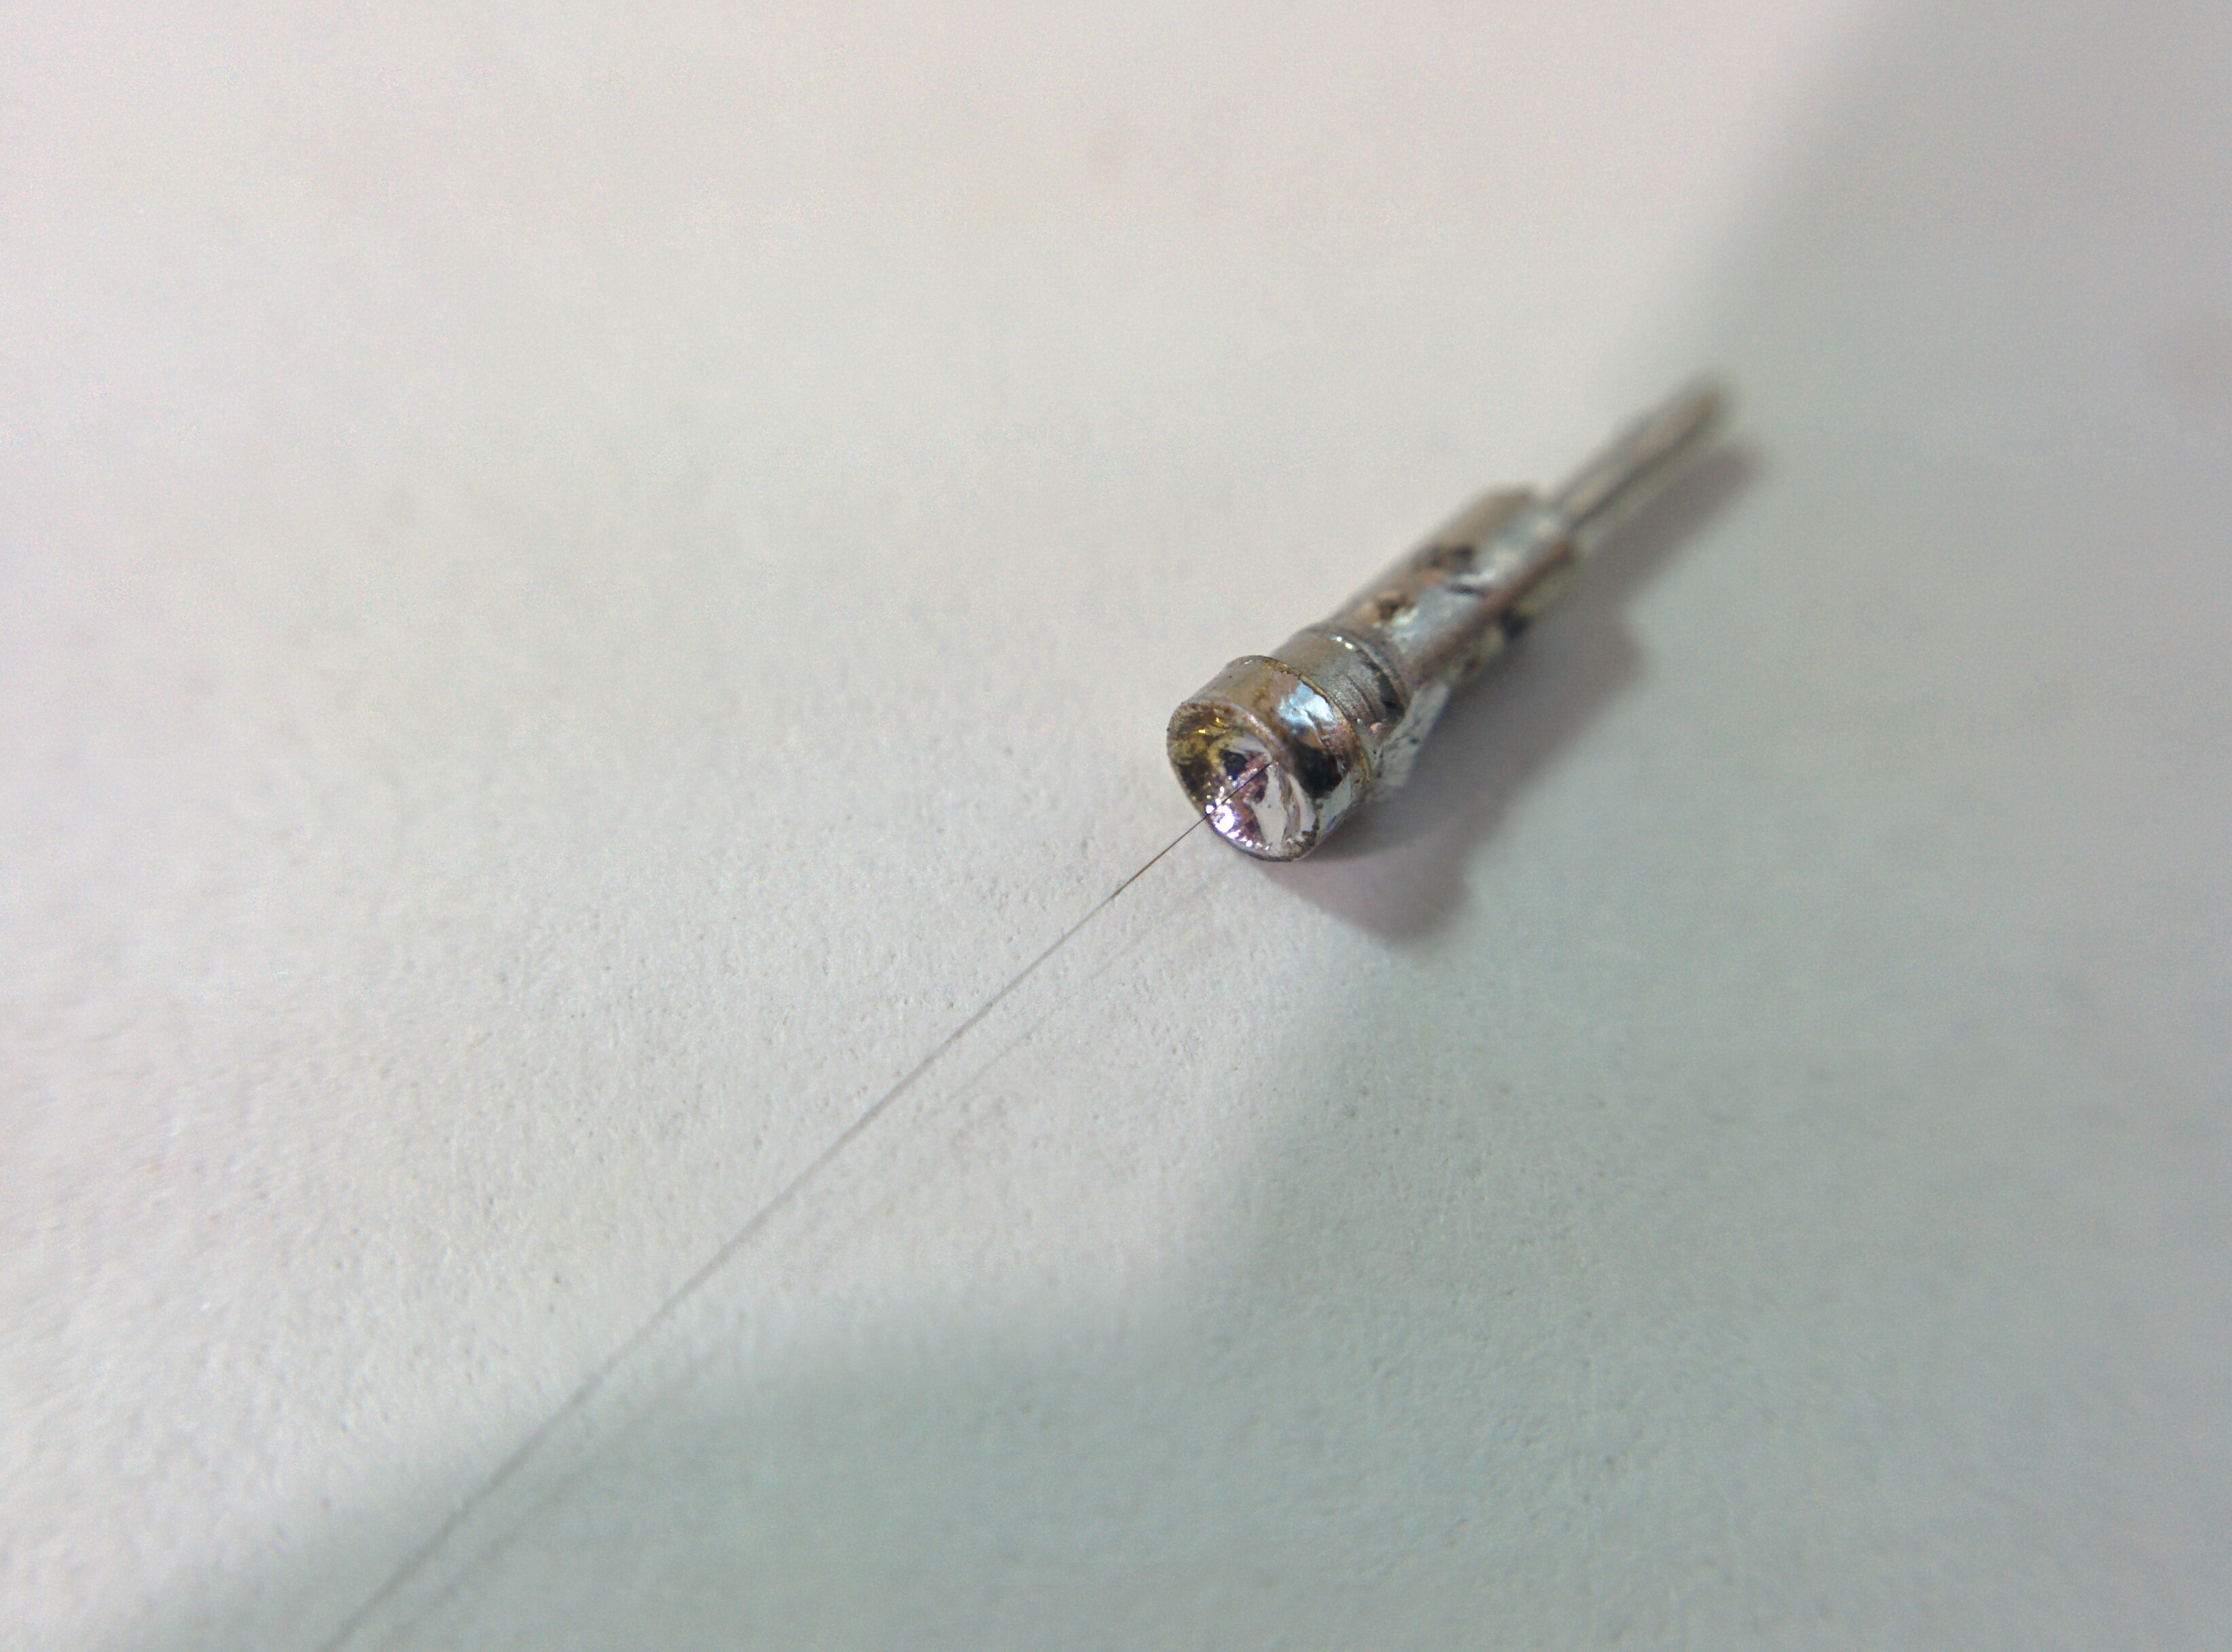
\includegraphics[trim = 200mm 20mm 150mm 150mm, clip, width=0.3\textwidth]{microelectrode.jpg}
\caption{}
\label{fig:2d}
\end{figure}

\def\s{0.5}
\def\left{70}
\def\bottom{120}
\def\right{50}
\def\top{30}
\begin{figure}
\centering
\begin{tikzpicture}
    \draw (0, 0) node[inner sep=0] {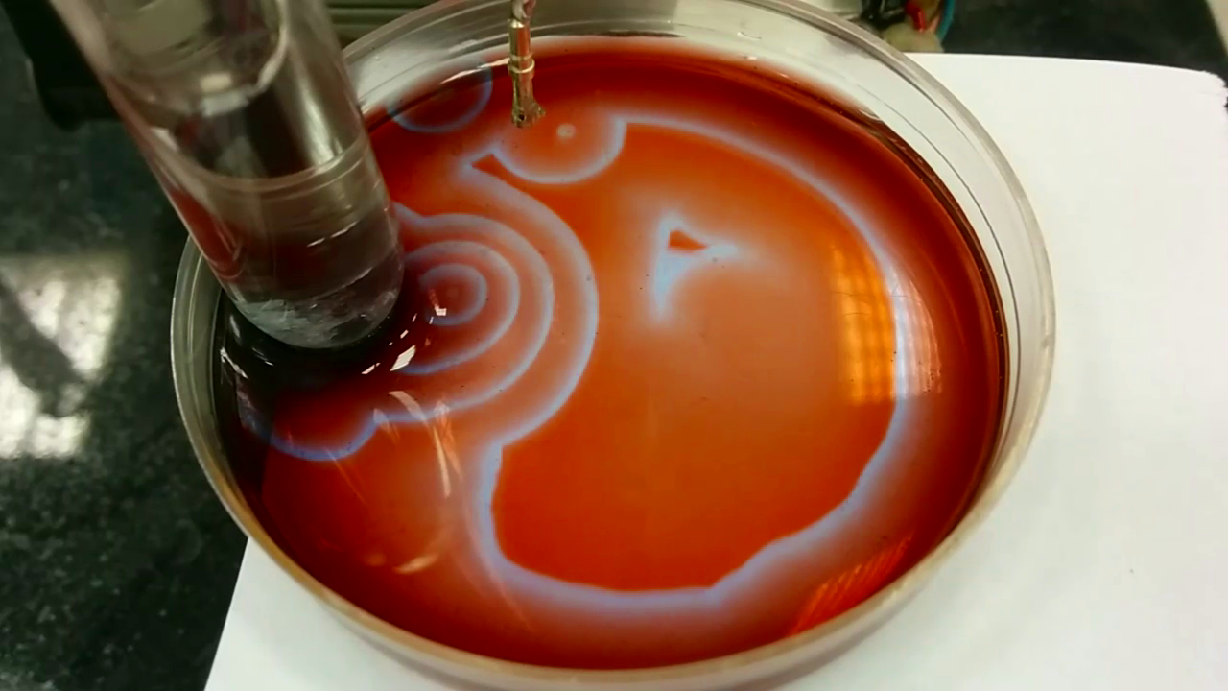
\includegraphics[trim = \left mm \bottom mm \right mm \top mm, clip, width=\s\textwidth]{0.png}};
    \draw (3.8, 1) node {a};
    \draw [green] (-1.1,-0.55) node[anchor=south] {\textbf{\large{•}}};
    \draw [blue] (0.2,-0.55) node[anchor=south] {\textbf{\large{•}}};
\end{tikzpicture}
%\begin{tikzpicture}
%    \draw (0, 0) node[inner sep=0] {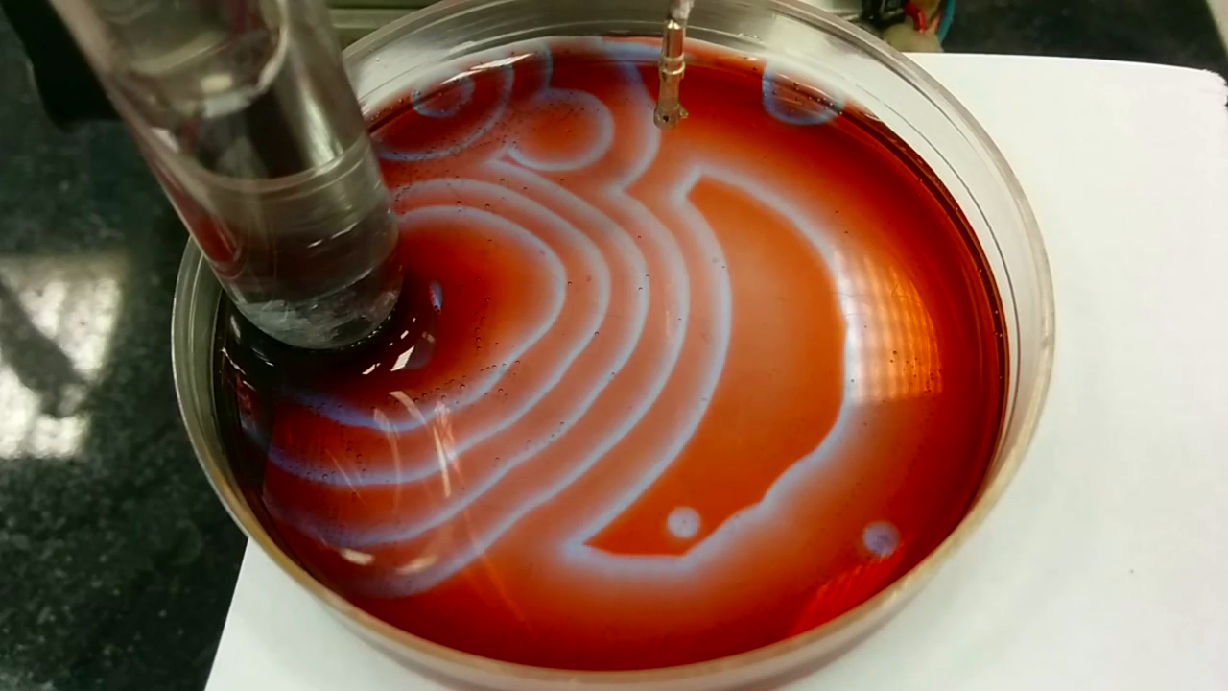
\includegraphics[trim = \left mm \bottom mm \right mm \top mm, clip, width=\s\textwidth]{right.png}};
%    \draw (3.8, 1) node {a};
%    \draw [green] (-1.1,-0.55) node[anchor=south] {\textbf{\large{•}}};
%    \draw [purple] (0.2,-0.55) node[anchor=south] {\textbf{\large{•}}};
%\end{tikzpicture}
\begin{tikzpicture}
    \draw (0, 0) node[inner sep=0] {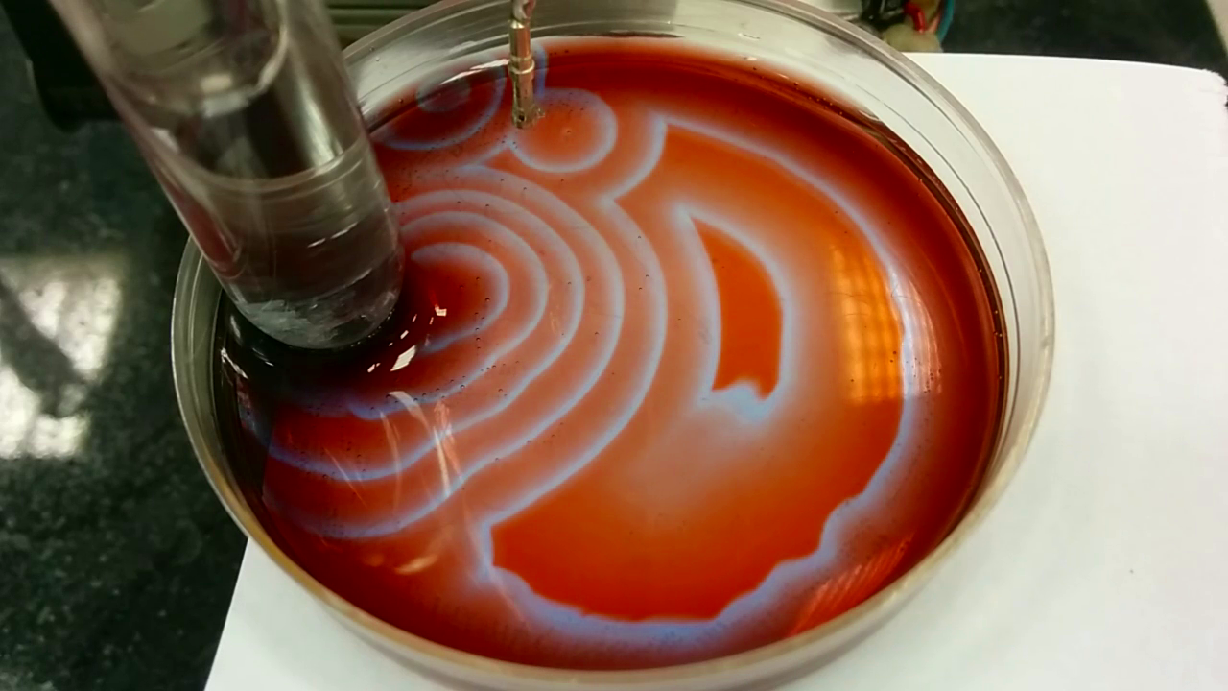
\includegraphics[trim = \left mm \bottom mm \right mm \top mm, clip, width=\s\textwidth]{1.png}};
    \draw (3.8, 1) node {b};
    \draw [green] (-1.1,-0.55) node[anchor=south] {\textbf{\large{•}}};
    \draw [blue] (0.2,-0.55) node[anchor=south] {\textbf{\large{•}}};

\end{tikzpicture}
\begin{tikzpicture}
    \draw (0, 0) node[inner sep=0] {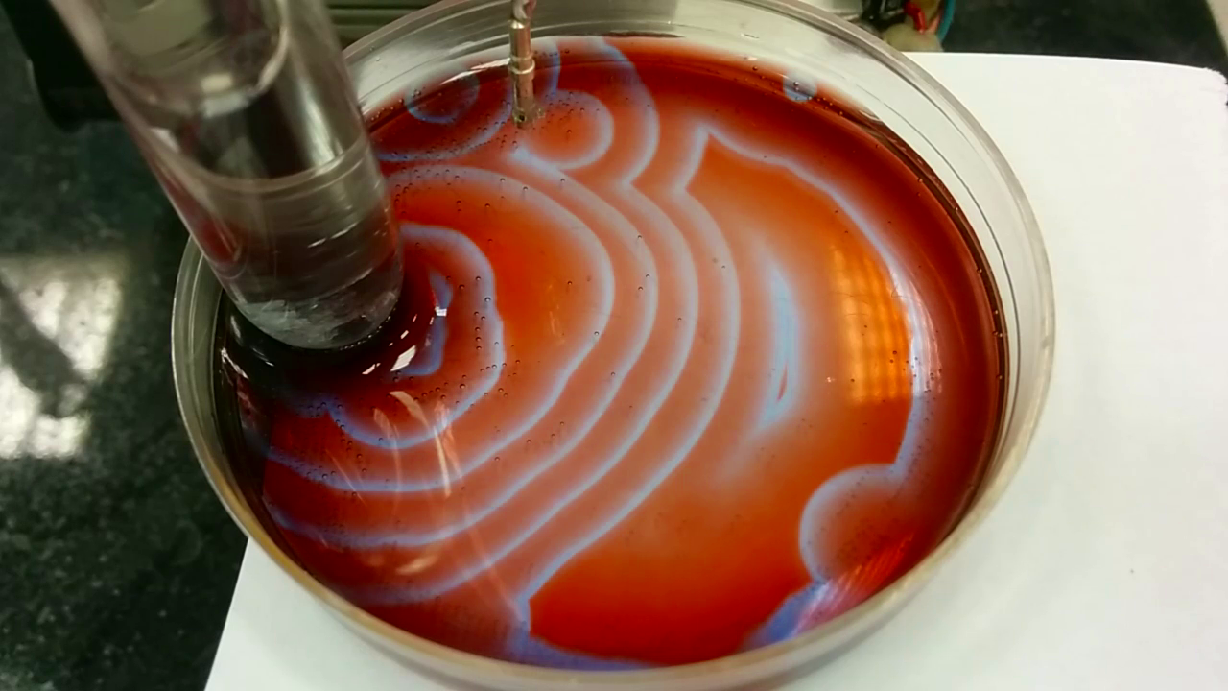
\includegraphics[trim = \left mm \bottom mm \right mm \top mm, clip, width=\s\textwidth]{2.png}};
    \draw (3.8, 1) node {c};
    \draw [green] (-1.1,-0.55) node[anchor=south] {\textbf{\large{•}}};
    \draw [blue] (0.2,-0.55) node[anchor=south] {\textbf{\large{•}}};

\end{tikzpicture}
\begin{tikzpicture}
    \draw (0, 0) node[inner sep=0] {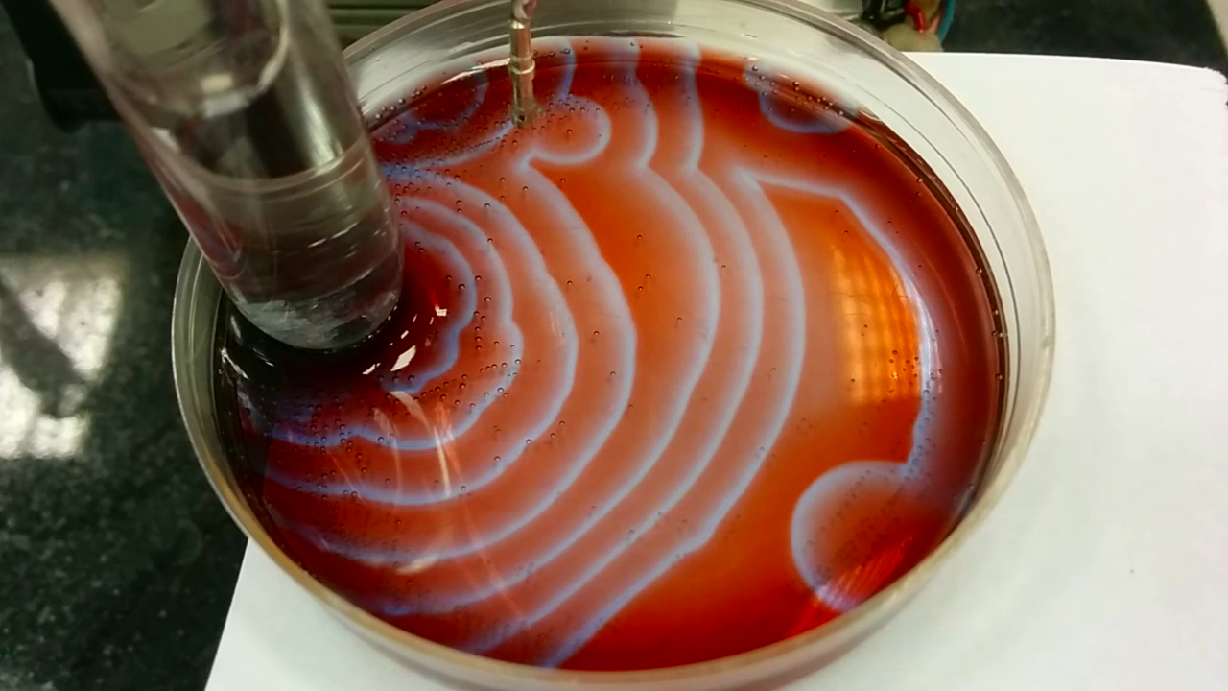
\includegraphics[trim = \left mm \bottom mm \right mm \top mm, clip, width=\s\textwidth]{3.png}};
    \draw (3.8, 1) node {d};
    \draw [green] (-1.1,-0.55) node[anchor=south] {\textbf{\large{•}}};
    \draw [blue] (0.2,-0.55) node[anchor=south] {\textbf{\large{•}}};

\end{tikzpicture}
\caption{Incomplete.}
\label{fig:grabs}
\end{figure}

%\begin{tikzpicture}
%  \begin{axis}
%    \addplot3[colormap/viridis, surf, very thick] table {17101308_st_lines.txt};
%    %\addplot3[color=black, surf, very thick] table {17101308_st_lines.txt};
%  \end{axis}
%\end{tikzpicture}


\section{Conclusions}

\section*{Acknowledgements}

\section*{References}

\begin{thebibliography}{5}
\bibitem{belousov} Belousov, B. P. "Sbornik Referatov po Radiatsionni Meditsine." Medgiz, Moscow 145 (1958).

\bibitem{fkn1} Noyes, Richard M., Richard Field, and Endre Kőrös. "Oscillations in chemical systems. I. Detailed mechanism in a system showing temporal oscillations." Journal of the American Chemical Society 94.4 (1972): 1394-1395.

\bibitem{fkn2} Field, Richard J., Endre Kőrös, and Richard M. Noyes. "Oscillations in chemical systems. II. Thorough analysis of temporal oscillation in the bromate-cerium-malonic acid system." Journal of the American Chemical Society 94.25 (1972): 8649-8664.

%\bibitem{hess1} Nagy-Ungvarai, Zs, et al. "Experimental study of spiral waves in the cerium-catalyzed Belousov-Zhabotinskii reaction." Journal of physical chemistry 94.24 (1990): 8677-8682.

\bibitem{hess2}Nagy-Ungvárai, Zs, H. Baumgärtl, and B. Hess. "Electrochemical detection of pattern formation in the Belousov-Zhabotinskii reaction." Chemical Physics Letters 168.6 (1990): 539-542. 

\bibitem{hess3}Nagy-Ungvárai, Zsuzsanna, and Benno Hess. "Control of dynamic pattern formation in the Belousov-Zhabotinsky reaction." Physica D: Nonlinear Phenomena 49.1-2 (1991): 33-39.

\bibitem{winfree} Winfree, Arthur T. The geometry of biological time. Vol. 12. Springer Science \& Business Media, 2001.

\end{thebibliography}


\end{document}
